% !TeX spellcheck = en_US

\documentclass[acmtog]{acmart}
\usepackage{amsmath}
\usepackage{multirow}
\usepackage{subfig}
\usepackage[acronym]{glossaries}
\usepackage{todonotes}
\usepackage{tikz}
\usepackage{graphicx}
\usepackage{makecell}


\AtBeginDocument{%
	\providecommand\BibTeX{{%
			Bib\TeX}}}

\setcopyright{acmcopyright}
\copyrightyear{2022}
\acmYear{2022}
\acmDOI{XXXXXXX.XXXXXXX}




%%
%% These commands are for a JOURNAL article.
\acmJournal{JACM}
\acmVolume{37}
\acmNumber{4}
\acmArticle{28}
\acmMonth{2}

\newacronym{wfs}{wfs}{Web Feature Service}
\newacronym{wps}{wps}{Web Processing Service}
\newacronym{res}{res}{resolution}
\newacronym{r}{r}{ratio}
\newacronym{al}{al}{all touched}
\newacronym{t}{t}{True}
\newacronym{f}{f}{False}
\newacronym{agg.}{agg.}{aggregated}
\newacronym{rel}{rel}{relative}
\newacronym{corr}{corr}{corrected}
\newacronym{MCDA}{MCDA}{multi-criteria decision analysis}

\begin{document}
	\title{Web Processing - Standardised GIS Analyses for Cable Route Planning}
	
	\author{Sebastian Heiden}
	\email{u38439@hs-harz.de}
	\affiliation{%
		\institution{Harz University of Applied Sciences}
		\streetaddress{Friedrichstrasse 57-59}
		\city{Wernigerode}
		\state{Saxony-Anhalt}
		\country{Germany}
		\postcode{38855}
	}
	
	
	\renewcommand{\shortauthors}{Heiden}
	
	\begin{abstract}
		The least cost paths for a power line route from a power station is computed to a power station further inland.
		Down sampling and clipping as studied as techniques to speed-up the computation.
		The path from clipped cost raster often matches the original path.
		The speed-up of the clipping can not be known before hand.
	\end{abstract}
	
	%%
	%% The code below is generated by the tool at https://dl.acm.org/ccs.cfm.
	%% Please copy and paste the code instead of the example below.
	%%
	\begin{CCSXML}
		<ccs2012>
		<concept>
		<concept_id>10010147.10010341</concept_id>
		<concept_desc>Computing methodologies~Modeling and simulation</concept_desc>
		<concept_significance>500</concept_significance>
		</concept>
		<concept>
		<concept_id>10002944.10011123.10011133</concept_id>
		<concept_desc>General and reference~Estimation</concept_desc>
		<concept_significance>100</concept_significance>
		</concept>
		</ccs2012>
	\end{CCSXML}
	
	\ccsdesc[500]{Computing methodologies~Modeling and simulation}
	\ccsdesc[100]{General and reference~Estimation}


	
	%%
	%% Keywords. The author(s) should pick words that accurately describe
	%% the work being presented. Separate the keywords with commas.
	\keywords{GIS, least cost path}
	
	\received{20 February 2007}
	\received[revised]{12 March 2009}
	\received[accepted]{5 June 2009}
	
	%%
	%% This command processes the author and affiliation and title
	%% information and builds the first part of the formatted document.
	\maketitle
	
	\section{Introduction}\label{sec:introduction}

	The German power system adds a lot of renewable energy sources in the north, because wind energy reaches highest efficiency with high wind speeds.
	At the same time old power plants e.g.\ nuclear, hard coal and lignite are going out off service~\cite{eser-frey_analyzing_2012}.
	These older power plants were mainly situated in southern and central Germany. 
	The power sink, which is industrial and private demand does not shift northwards.
	Therefore, the renewable energies have to be transported from north to south which increases the congestion in the power grid. 
	The amount of offshore wind power, that the German energy system can use, can be greatly increased by adding new power lines~\cite{leuthold_nodal_2005}.
	
	But for building power lines, finding the shortest path is not sufficient.
	Additional parameters also have to be taken into consideration.
	As the steepness of a road or the soil, play an important role for the building cost of a road or pipeline~\cite{suleiman_optimal_2015}.
	For planing the additional routes for a power grid, further aspects as legal regulations and acceptance
	by the local population have to be taken in consideration.
	Also technical aspects, as the effects on the grid stability are further points take into consideration~\cite{schafer_understanding_2022}.
	
	Due to the increasing need for renewable energy wind offshore wind turbines supply 5.5~\% annual percentage in 2020 of the German energy mix~\cite{noauthor_nettostromerzeugung_2021}.

	Other methods as the \acrfull{MCDA}  consider further aspects as stakeholder, experts, public and decision maker~\cite{bertsch_participatory_2016} (see section~\ref{sec:related-works}).
	
	For planning a possible route for a power line the least cost path algorithm is applied.
	The least cost path algorithm is a Dijkstra algorithm~\cite{dijkstra_note_1959} applied on a raster map.
	The vertices of the graph are the pixel centers, that are connected to the eight neighboring pixel centers via the edges.
	This enables to find routes on graphs that are not predefined like road notworks.
	The weights of the edges are the local costs to travel from one pixel center to the neighboring pixel center.
	The costs might be physical costs, as the local slope, but also can be composed on other factors as the acceptance rate for the land usage of a given class.
	The least cost path algorithm consists of at least two sequential steps.
	1) The first step is to aggregate the costs of traveling from the starting point to a given set of end points.
	This step generates the aggregated cost raster of traveling from the starting point to any point of the cost raster.
	2) In the next step the back tracking, the route of the actual least cost path is calculated.
	For each ending point the path via the lowest cost neighbor is taken until arriving at the starting point.
	
	Some implementations switch the role of start and ending points, so that either many starting points and one end point, or one end point and many endpoints can be used.
	In some implementation there is a extra step between 1) and 2) that calculates cost-weight direction raster, that encodes the direction of the shortest
	path to the starting point as integer values.

	\section{Methods}\label{sec:methods}
	% !TeX spellcheck = en_GB

The least cost path algorithm is used to plan a possible route for a power line.
The least cost path algorithm is a Dijkstra algorithm~\cite{dijkstra_note_1959} applied on a raster map.
The vertices of the graph are the pixel centres, that are connected to the eight neighbouring pixel centres via the edges.
This makes it possible to find routes on graphs that are not predefined, such as road networks.
The weights of the edges are the local costs of travel from one pixel center to the neighbouring pixel center.
The costs can be physical costs, such as the local slope, but also can be composed of other factors as the acceptance rate to transverse a given land usage.
The Least Cost Path algorithm consists of at least two successive steps.
1) The first step is to aggregate the costs of travelling from the starting point to a given set of end points.
This step generates the aggregated cost raster of travelling from the starting point to any point of the cost raster.
2) In the next step the backtracking, the route of the actual Least Cost Path is calculated.
For each end point the path via the lowest cost neighbour is taken until the starting point is reached.

Some implementations switch the role of start and ending points, so that either many start points and one single end point, or one single end point and many end points can be used.
In some implementation there is an extra step between 1) and 2) that calculates cost-weight direction raster, that encodes the direction of the shortest
path to the starting point as integer values.

We retrieve a set of different spacial data-sets from  public sources as a basis for creating the cost raster.
The study area are the counties of Cuxhaven and Osterholz in the state of Lower Saxony, Germany.
Areas protected by different European and National conservation laws are provided by the German Environment Agency
as \acrfull{wfs}~\cite{noauthor_schutzgebiete_2015}.

The national land coverage (ATKIS) with a scale of 1:250000 are provided by the Federal Agency for Cartography
and Geodesy~\cite{noauthor_digitales_2021}.
The national power grid (tags: 'power': line) has been retrieved via OpenStreetMap~\cite{boeing_osmnx_2017}.
Local data as houses at Level of Detail 1 are provided by the State Office for Geoinformation and Land Surveying of
Lower Saxony~\cite{noauthor_opengeodatani_2022}.
In addition, local planning geodata for the land use are taken
from 'Metropolplaner' (Planning data Lower Saxony \& Bremen)~\cite{noauthor_metropolplaner_2022}.

PyWPS~\cite{noauthor_welcome_2016} is used to provide the least cost path algorithm as a \acrfull{wps} in combination with flask~\cite{noauthor_flask_nodate}.
As client Birdy~\cite{noauthor_birdy_nodate} connects to the \acrshort{wps}, sends the cost raster and receives the resulting least cost path.
The initial implementation of the Least Cost Path algorithm is based on the implementation for the QGIS-Plugin
'Least Cost Path'~\cite{noauthor_leastcostpathdijkstra_algorithmpy_2022} in version 1.0, but refactored to optionally export the aggregated costs.

To computed intermediate cost cost raster the different layers of the different entities are optionally filtered, buffered and then rasterised.
Filtering the layers of the vector files for special attributes enables further differentiation.
For examples, it is possible to differentiate between heath and uncultivated land in the land cover.
Adding a buffer can be used either to convert a line object such as power lines and roads into a polygon (with the
correct physical width), or to add minimum distance from an existing of planed area to the new power line.
Each of theses intermediate rasters are given a weight (cost) which expresses the cost of using land covered by this layer.
In the final cost raster costs of all intermediate rasters are aggregated with the maximum function.
Thus, an area covered by several layers is uniformly associated with the highest cost.
Any place in the study area, that is not covered by any layer and thus does not yet have a weight, is given the default cost.

The costs have been grouped into five different levels~(see table~\ref{tab:1}), starting from \textit{Preferential} areas with
very low costs, via \textit{No restriction}s, which is the default, used when no other layers are covering the local area,
to \textit{Restricted}, \textit{Strongly Restricted} and \textit{Prohibited} areas with high costs.
These higher costs resemble the degree to which a place with this cost should be avoided, while routing the path.
The ratio of the higher costs to the lower costs directly translates into the additional detour in pixels
the algorithm is willing to go.
Thus, as \textit{prohibited} areas describe a legal obligation, not to use these areas or only to the utmost minimum,
the weight that resembles the costs for these types of areas, is set especially high.\\

All these layers are provided as vectors.
The Least Cost Path algorithm uses raster data.
Rasterisation transforms a vector into a raster.
Rasterisation can be done in two different ways.
In both ways, the rasterisation can be imaged, as the old vector is superimposed on the new raster grid with the new
given resolution and the new affine transformation and the coordinate reference system of the vector.
Both rasterisation techniques differ in the selection of the pixel, that describe the original polygon.
The pixels can be selected, if either the centre of that pixel is overlapped
by the geo-object, or any part of the pixel is overlaid.
Setting all touched to True, implies the version with any part of the pixel selected.
The version where an overlapped pixel centre is require is setting the parameter all touched to False.
All touched set to False is considered the default (see figure~\ref{fig:alltouched}).
\begin{figure}[!ht]
	\centering

	\resizebox{8cm}{!}{
		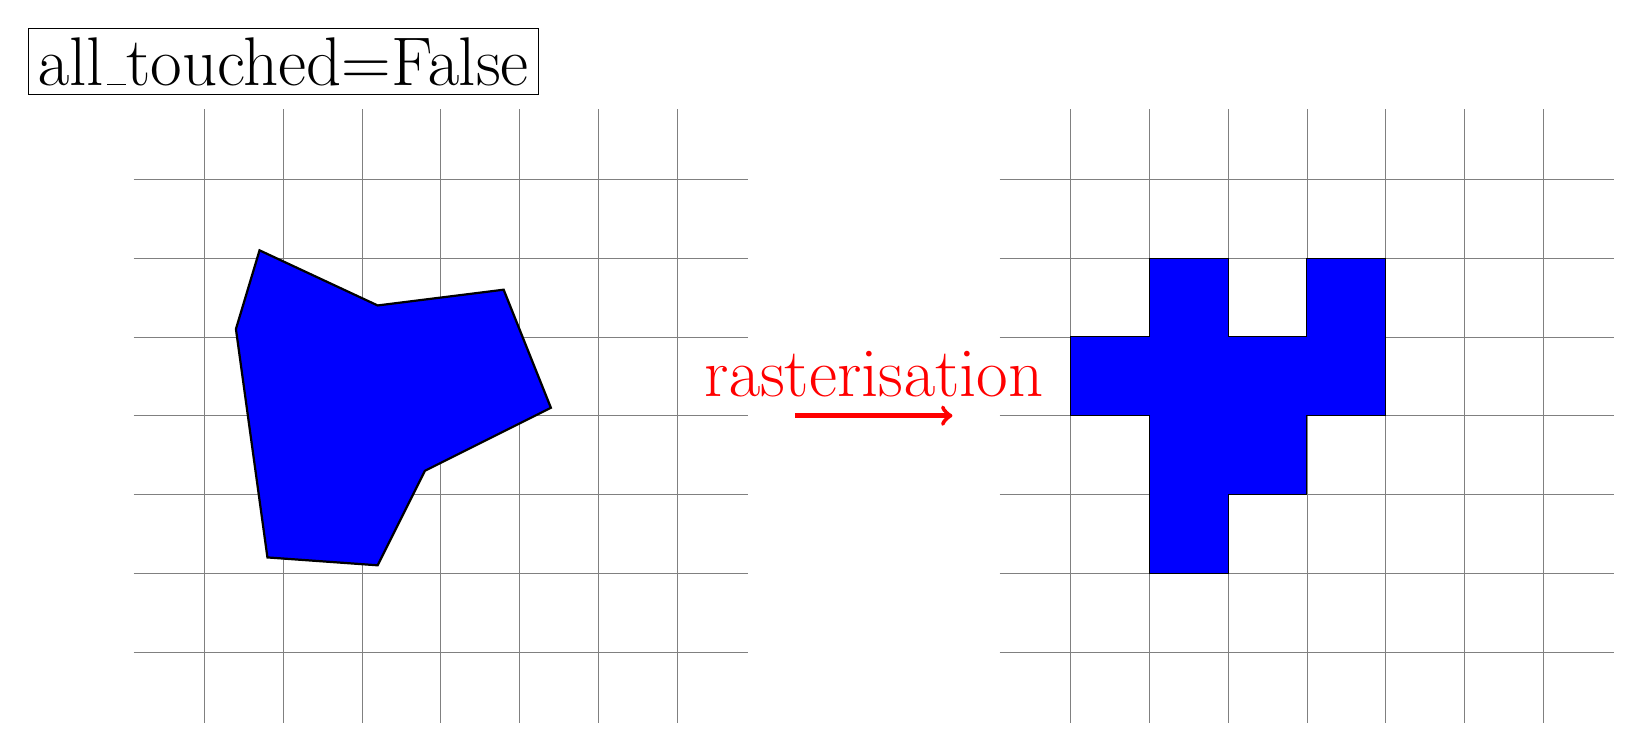
\begin{tikzpicture}
			\node[draw] at (0,6.5) {\Huge all\_touched=False};
			\draw[step=1cm,gray,very thin] (-1.9,-1.9) grid (5.9,5.9);
			\draw[fill=blue, thick] (-0.2, 0.2)--(-0.6, 3.1)--(-0.3,4.1)--(1.2,3.4)--(2.8,3.6)--(3.2, 2.6)--(3.4, 2.1)--(1.8,1.3)--(1.2, 0.1)--cycle;

			\draw[ultra thick,->, red] (6.5, 2) --node[above=1mm] {\Huge rasterisation} (8.5, 2);

			\draw[step=1cm,gray,very thin] (9.1,-1.9) grid (16.9,5.9);
			\draw[fill=blue] (11,0)--(11,2)--(10,2)--(10,3)--(11,3)--(11,4)--(12,4)--(12,3)--(13,3)--(13,4)--(14,4)--(14,2)--(13,2)--(13,1)--(12,1)--(12,0)--cycle;
		\end{tikzpicture}%
	}%
	\vspace*{5mm}
	\resizebox{8cm}{!}{
		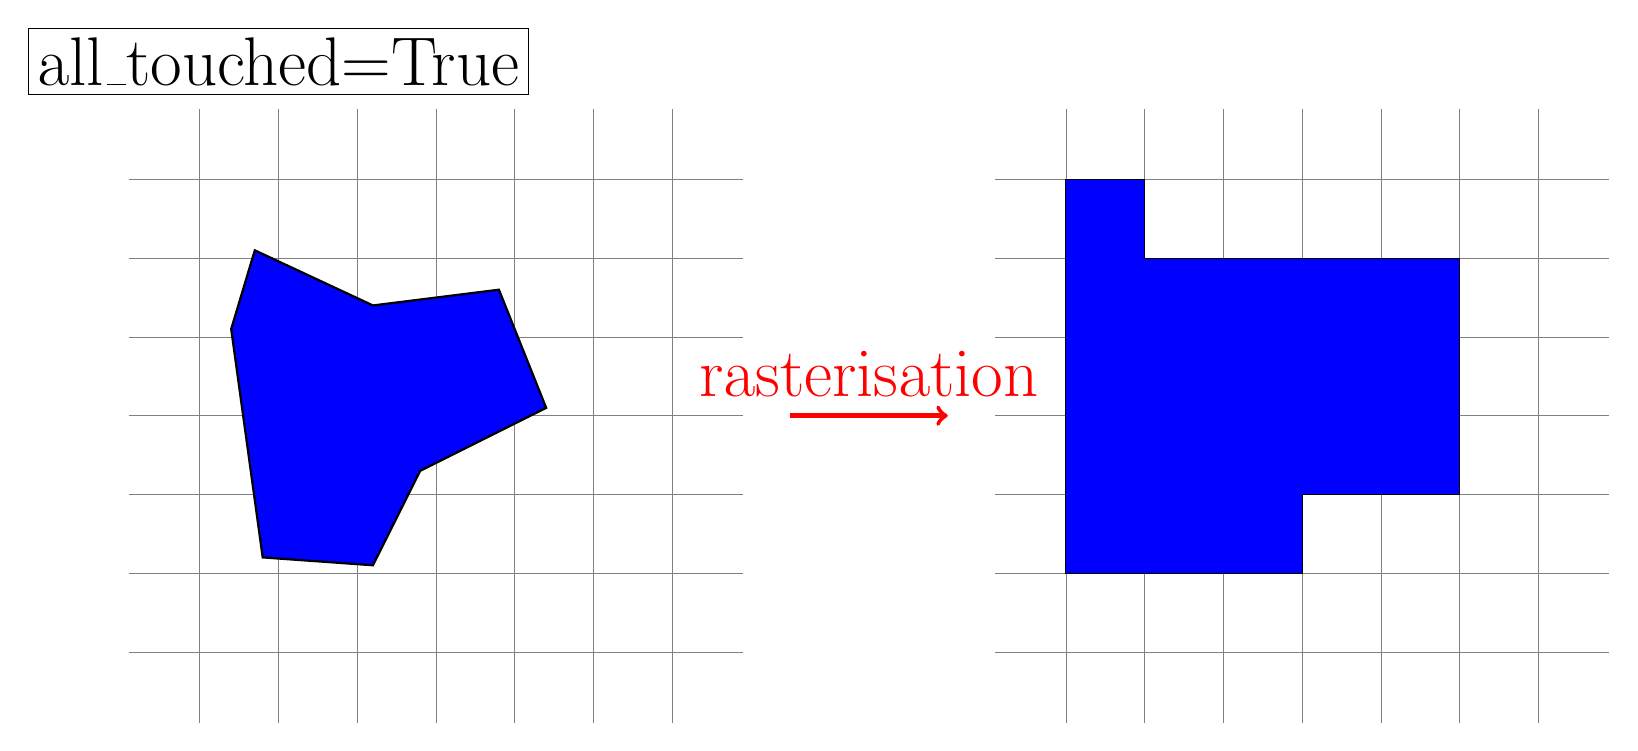
\begin{tikzpicture}
			\node[draw] at (0,6.5) {\Huge all\_touched=True};
			\draw[step=1cm,gray,very thin] (-1.9,-1.9) grid (5.9,5.9);
			\draw[fill=blue, thick] (-0.2, 0.2)--(-0.6, 3.1)--(-0.3,4.1)--(1.2,3.4)--(2.8,3.6)--(3.2, 2.6)--(3.4, 2.1)--(1.8,1.3)--(1.2, 0.1)--cycle;

			\draw[ultra thick,->, red] (6.5, 2) --node[above=1mm] {\Huge rasterisation} (8.5, 2);

			\draw[step=1cm,gray,very thin] (9.1,-1.9) grid (16.9,5.9);
			\draw[fill=blue] (10,0)--(10,5)--(11,5)--(11,4)--(15,4)--(15,1)--(13,1)--(13,0)--cycle;
		\end{tikzpicture}%
	}%
	\caption{Graphical example for rasterise a vector (left blue), to a raster (right blue) with either all touched set to False (above), or True (below).}
	\label{fig:alltouched}

\end{figure}

\begin{table}[h!]
	\caption{Used levels of costs, the applied numerical equivalent and example layer this cost have been used for.}
	\label{tab:1}
	\centering
	\begin{tabular}{ l  r  l }
		Cost Level 			& Cost 					& Example\\
		\hline
		Prohibited 			& 500					& \makecell[lt]{Conversation areas as\\ National Parks, Buildings} \\
		Strongly Restricted & 10 					& \makecell[lt]{Conversation areas as Bird Reserve} \\
		Restricted 			& 5						& \makecell[lt]{Protected Landscape Area,\\ Industrial Areas, motorway, railway} \\
		No Restriction 		& 0.5					& Default\\
		Preferential 		& 0.1					& \makecell[lt]{Power Grid,\\ Motorway and Railway Buffers}\\
	\end{tabular}
\end{table}

The complete list of layers and the applied processing steps, can be found in \textbf{Supplement S1}.

All three steps of the generation of the least cost path: generation of the cost raster, aggregation and backtracking is shown with an example for a cost raster of 50~m resolution and all touched set to False (see \ref{fig:costs2path}).

The chosen implementation applies early stopping.
Therefore, the costs for points that are not needed to try to connect to the end point are not aggregated (see figure \ref{fig:aggregation}).
After finding an aggregated cost for every end point, the aggregation stops and the backtracking starts.
Because the path ends at a power transformer, which is a building type, the paths ends at in a \textit{Prohibited} area.
Therefore, areas even further away from the starting point have been explored first.

\begin{figure}
	\centering
	
	\subfloat[\centering Cost Raster.]{{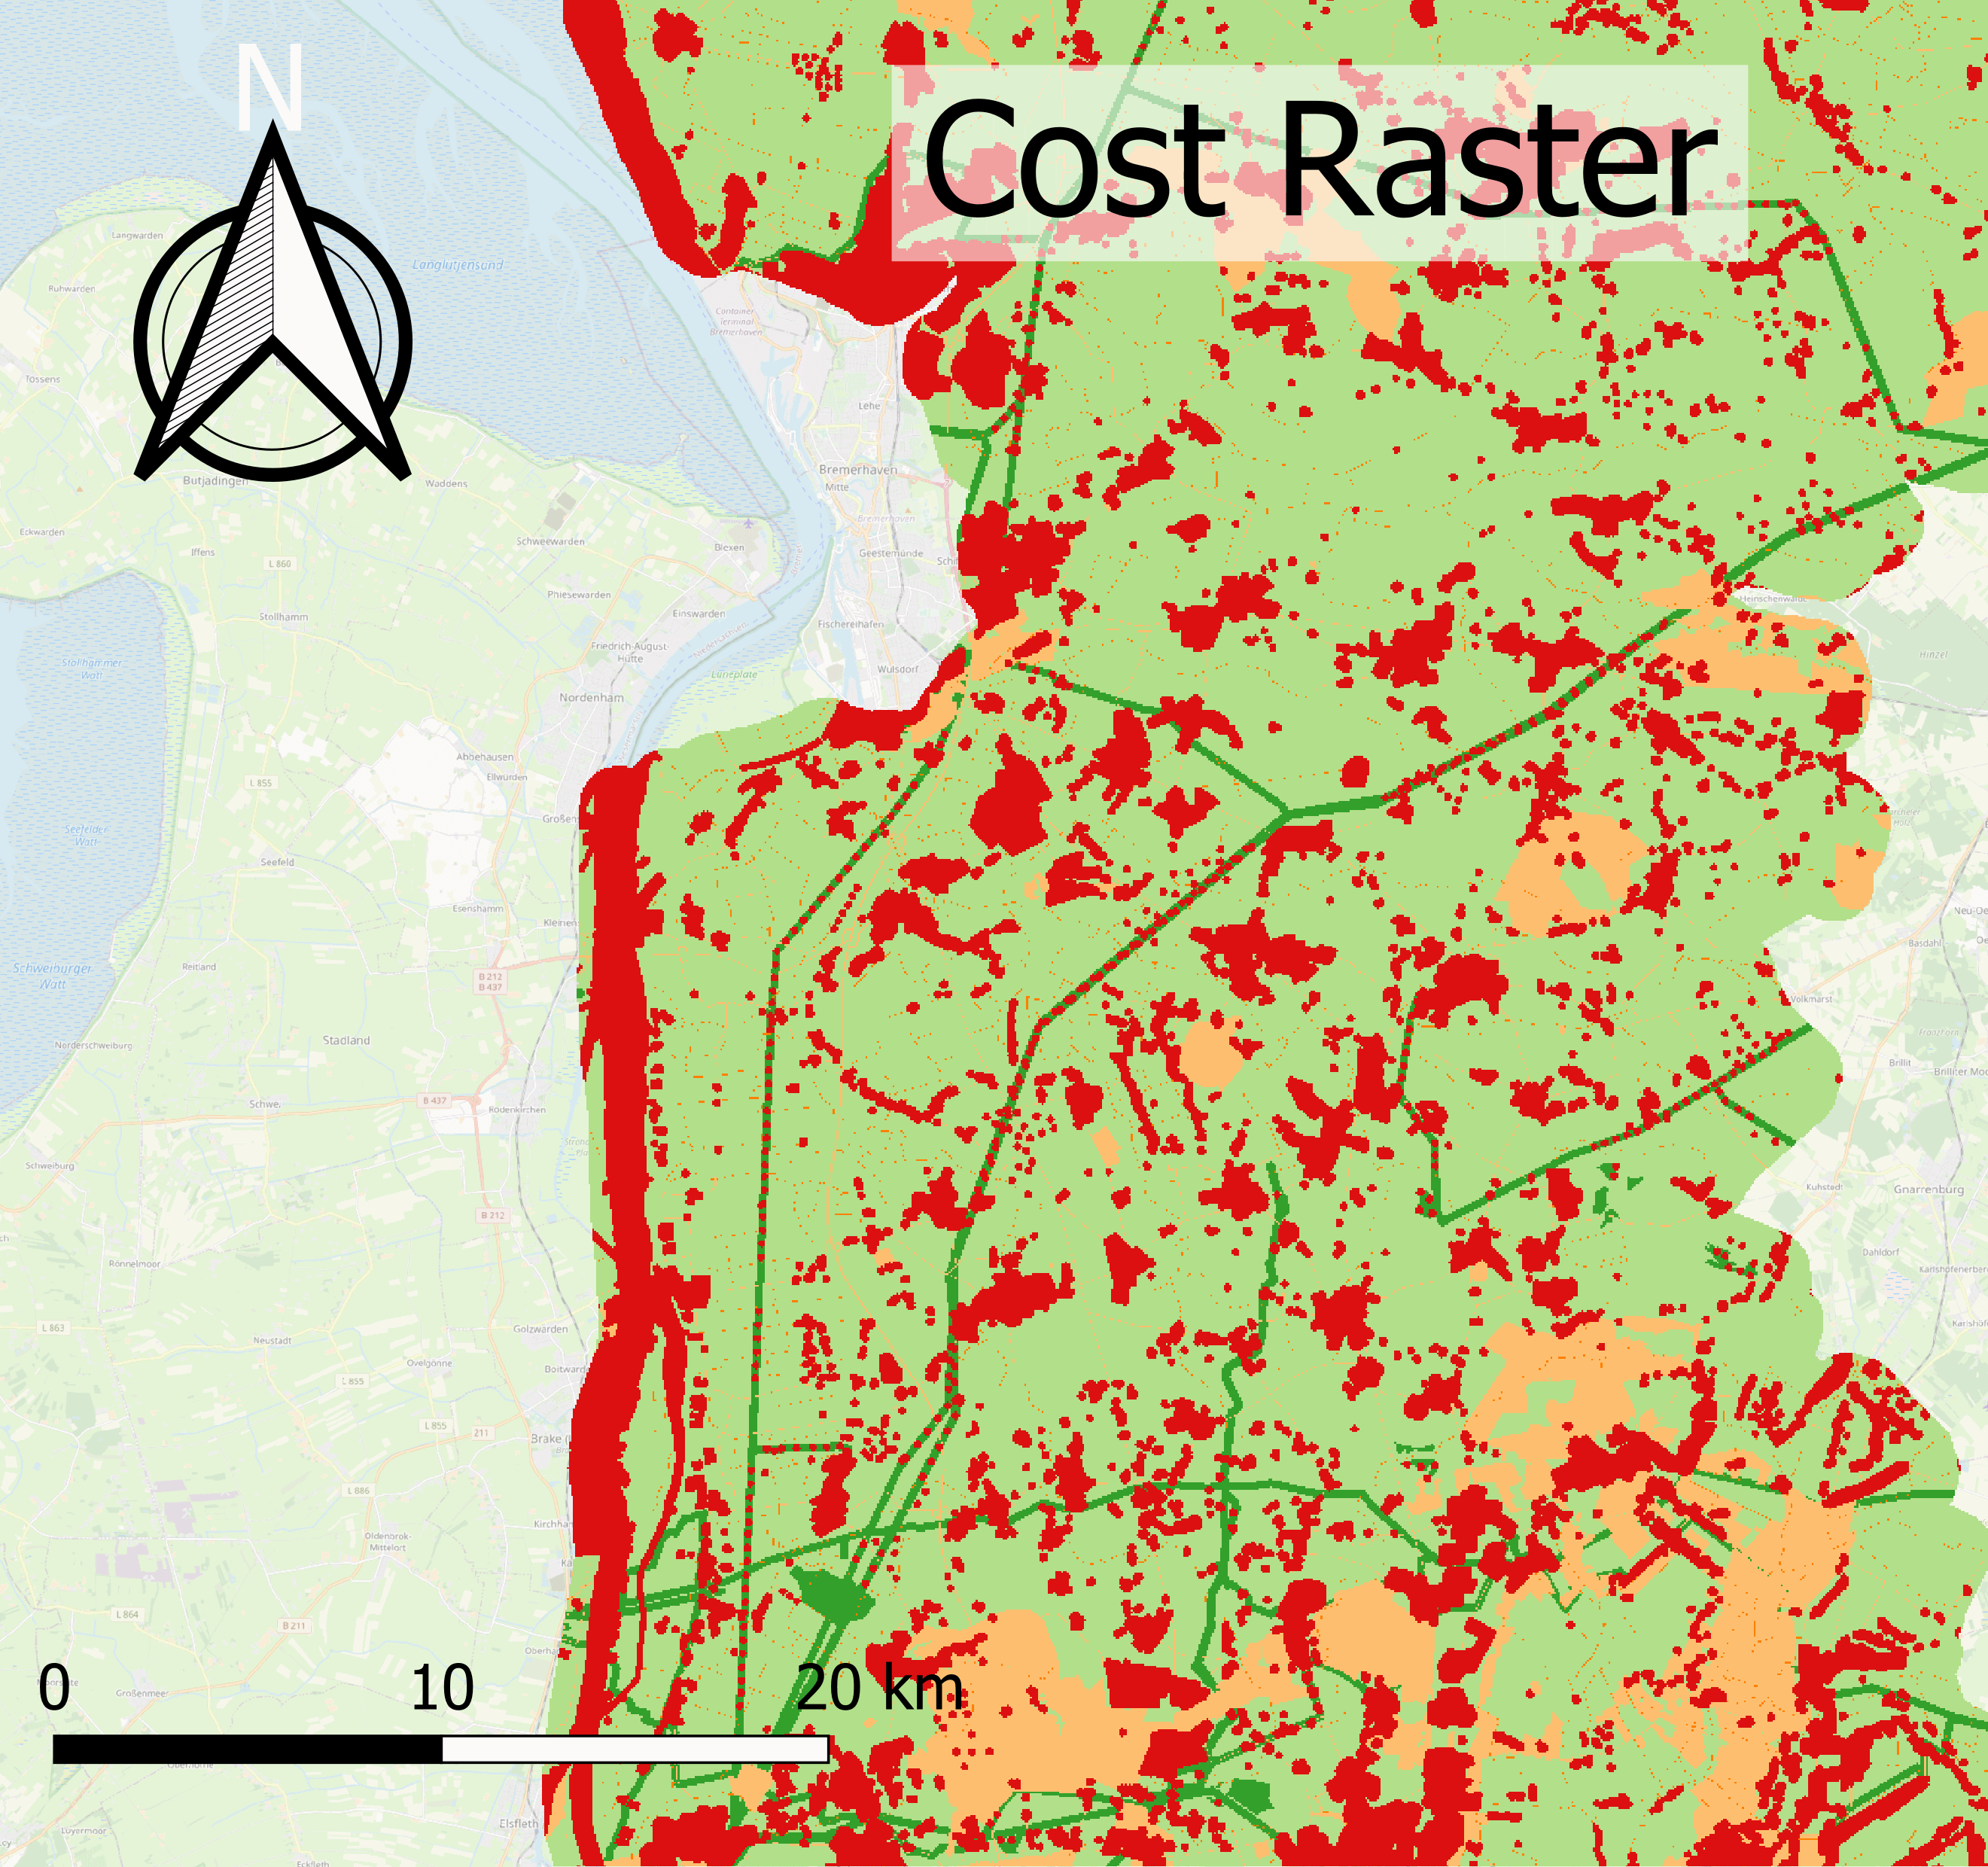
\includegraphics[width=.30\linewidth]{./images/CostRasterExample_cut.png} }}%
	\enskip
	\subfloat[\centering Aggregated Cost Raster.]{{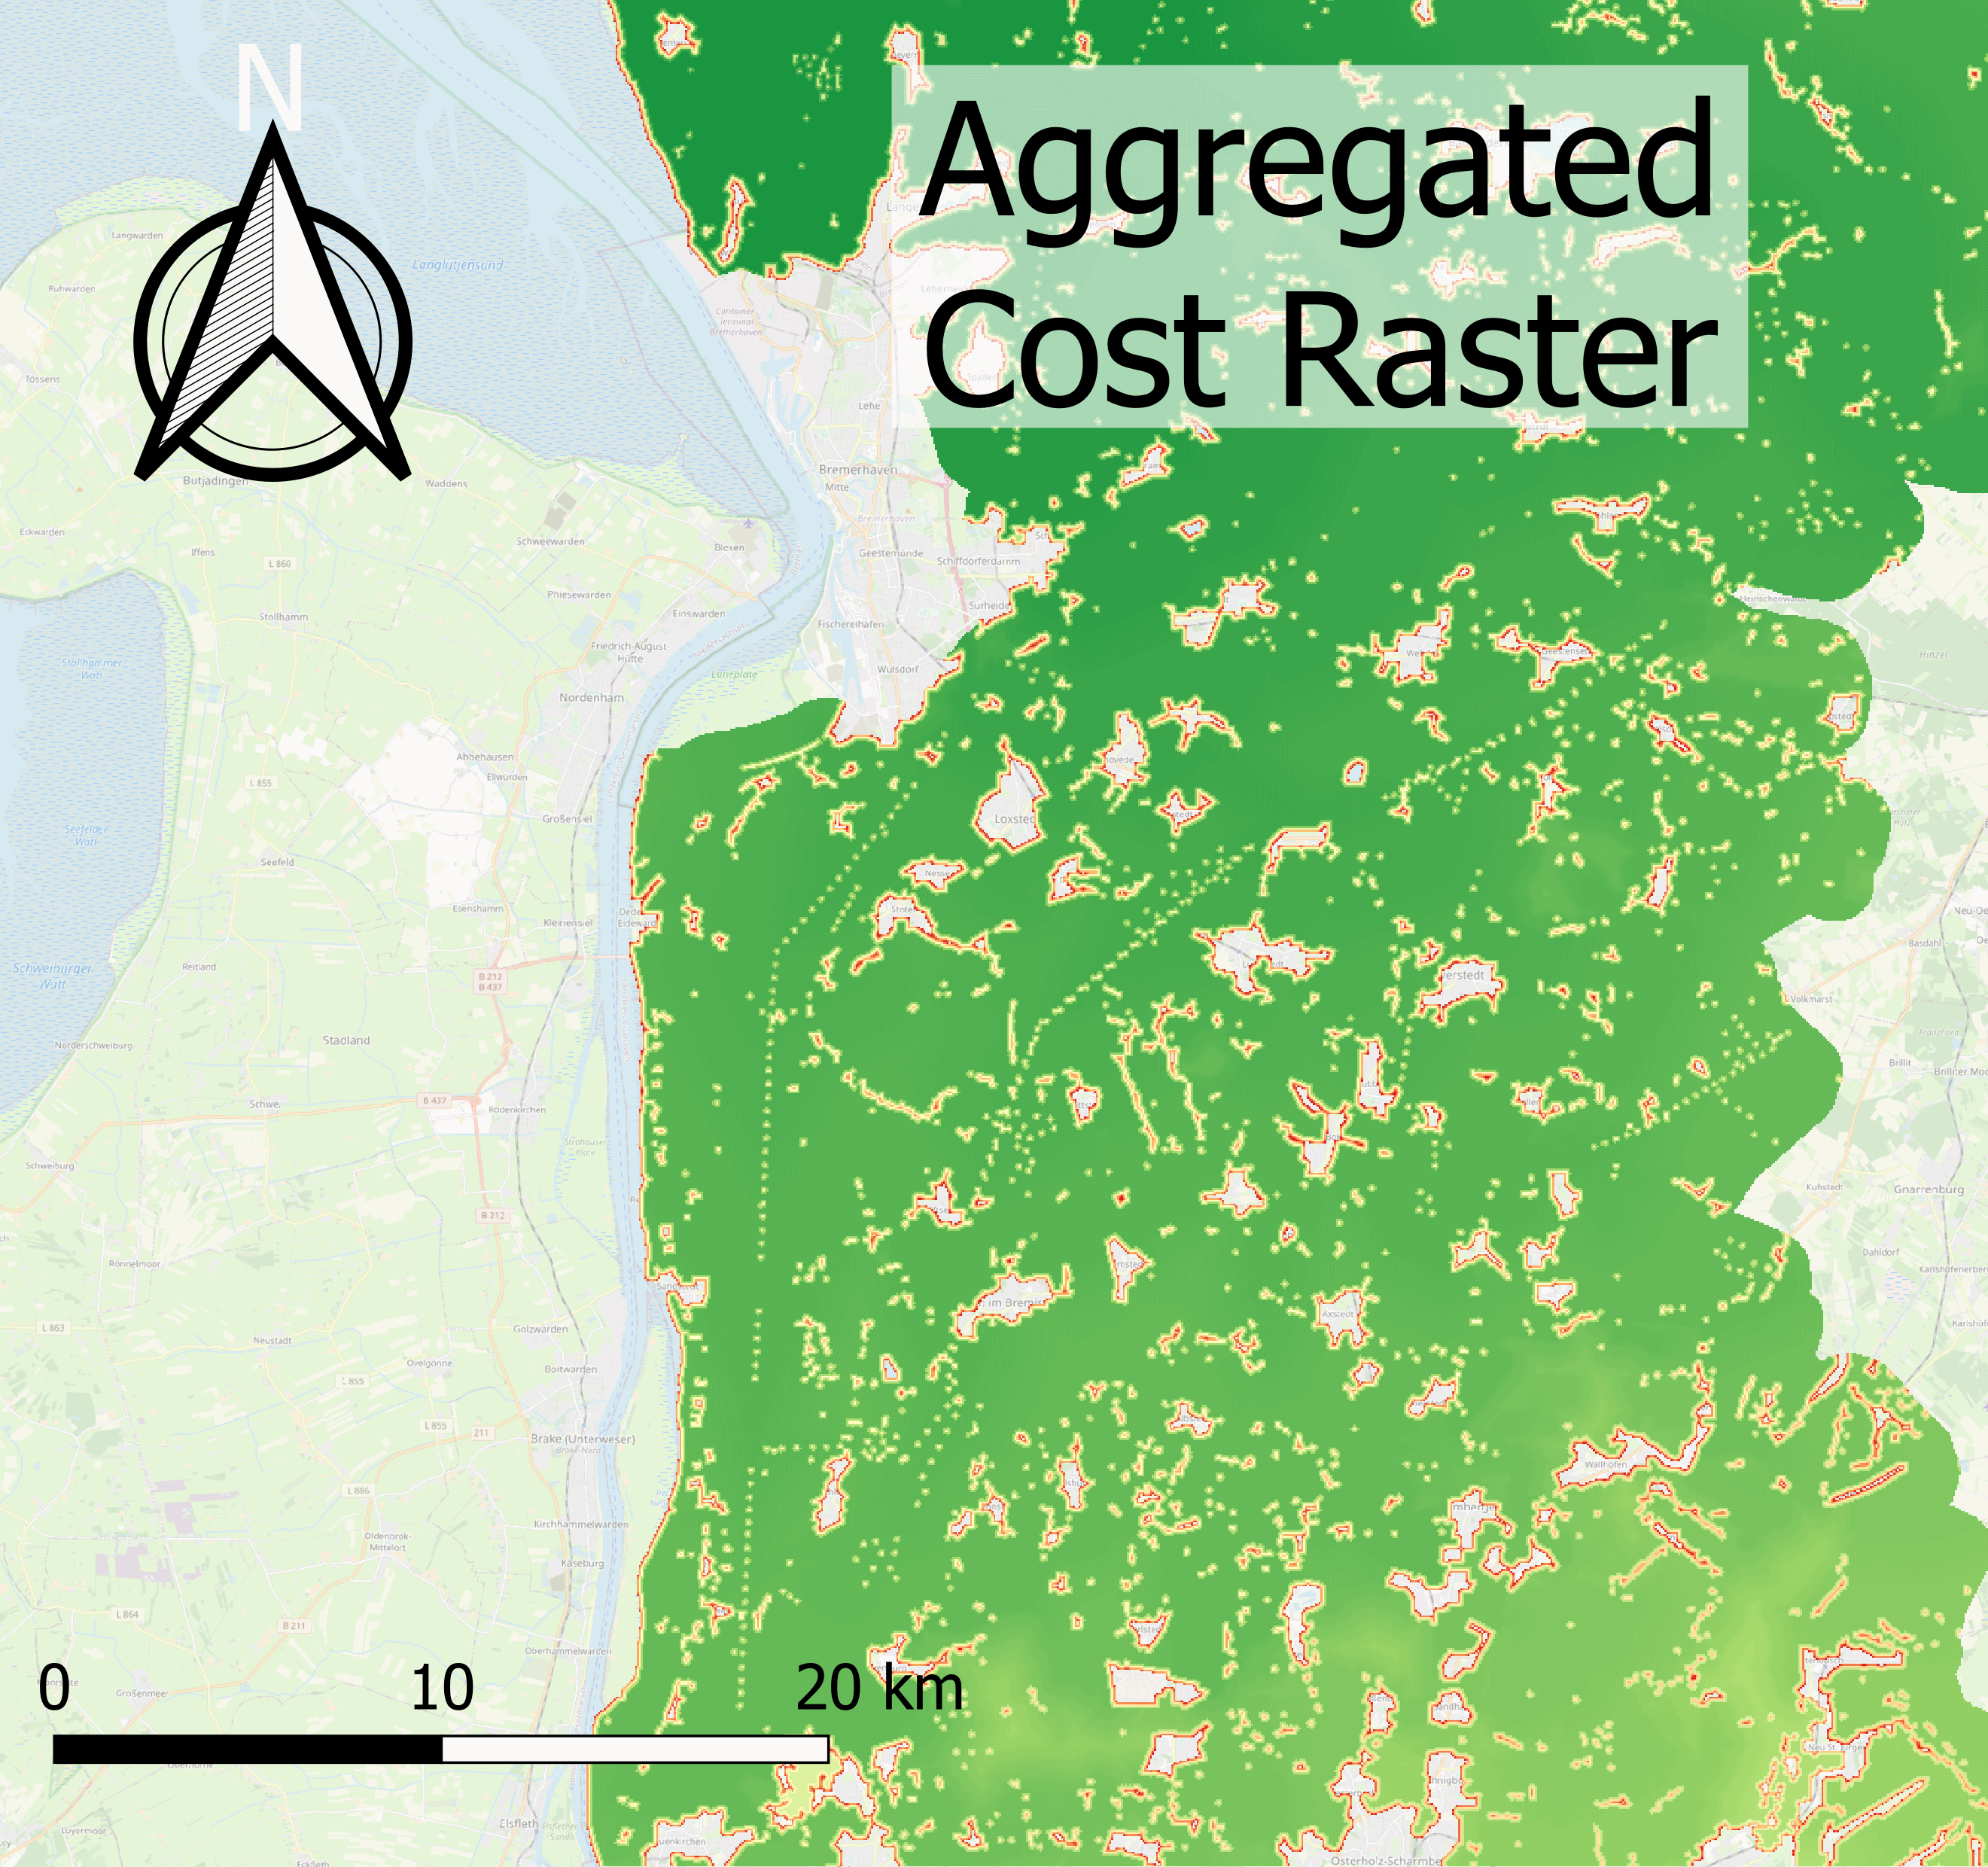
\includegraphics[width=.30\linewidth]{./images/AggregatedCosts_cut.png} \label{fig:aggregation}}}%
	\enskip
	\subfloat[\centering Least Cost Path.]{{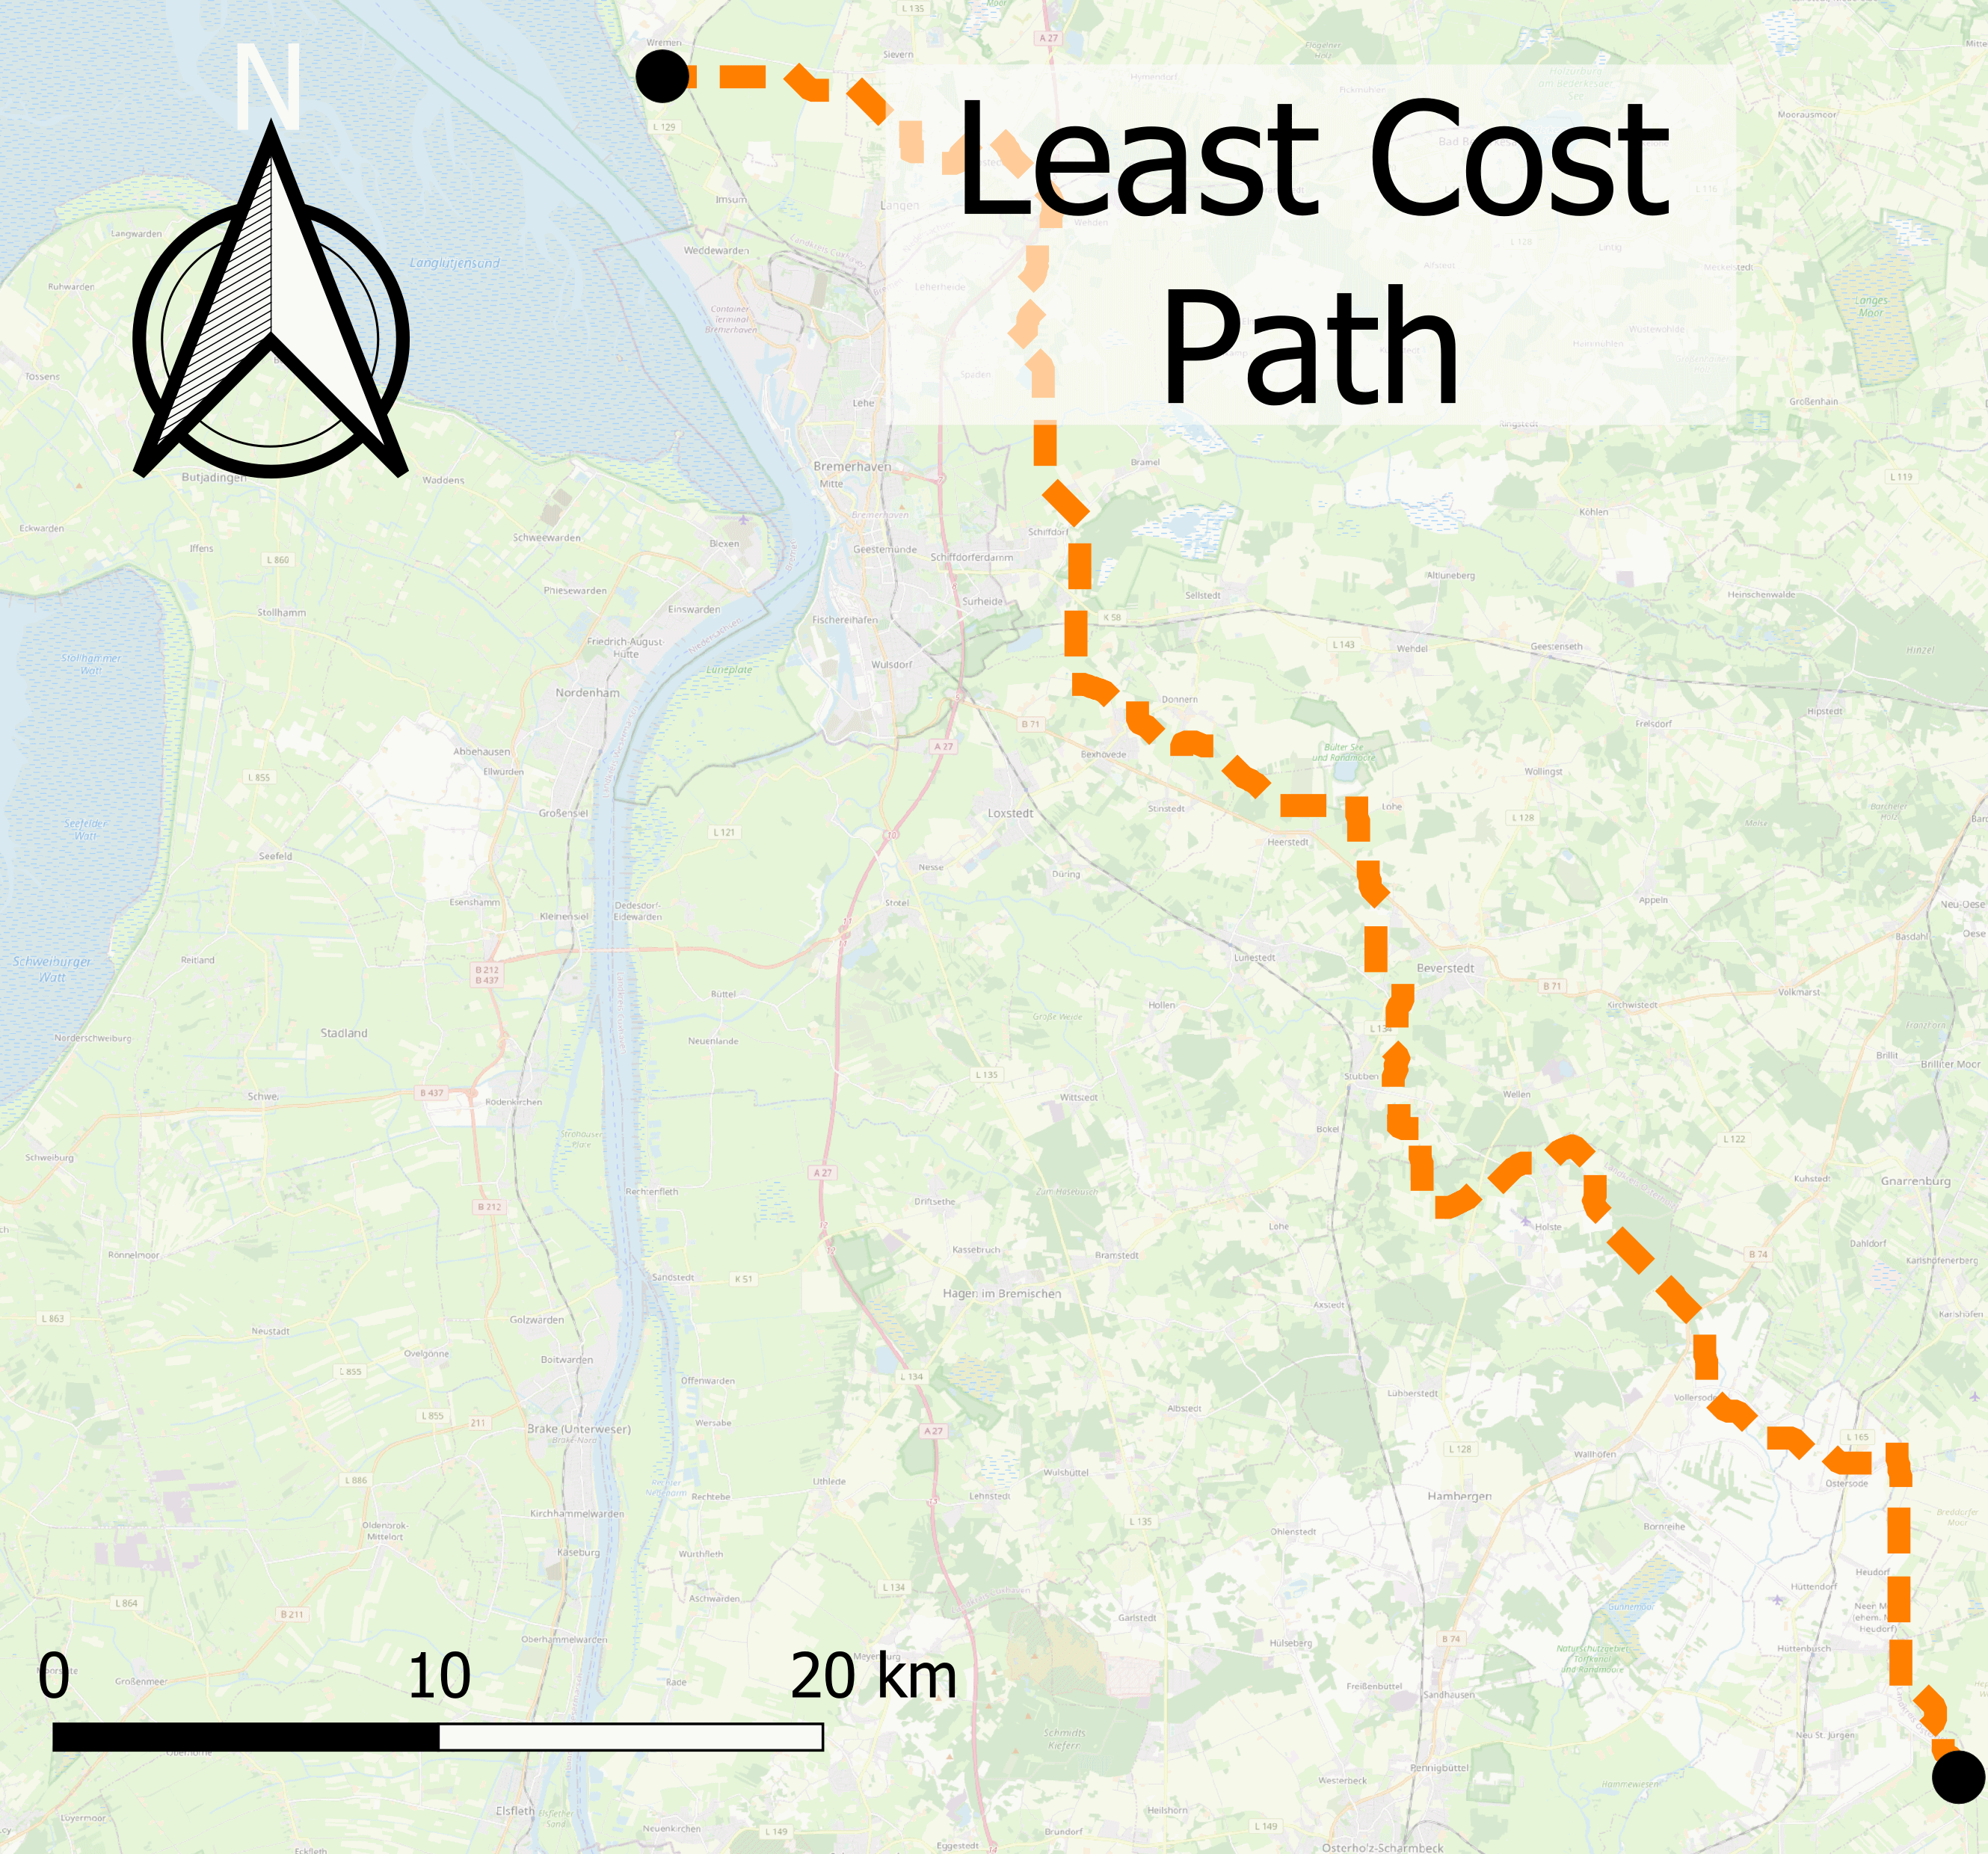
\includegraphics[width=.30\linewidth]{./images/LeastCostPathExample_cut.png} }}%

	\caption{Figures of the cost raster and the resulting aggregated costs and the Least Cost Path for a resolution of 50~m, all touched set to False.}
	\label{fig:costs2path}
\end{figure}

	

%% Aggregation is implemented in a priority queue. 
%% Hence a point with a lower cost is evaluated earlier as a starting position to evaluate the cost of its neighbours, than a point with higher cost.


For low resolution rasterisation with all touched set to True, will show every detail, but the objects are enlarged.
When all touched is to False the object only appears, when the is situated at the pixel centre.
Thus, this might be used as surrogate, that expresses the likelihood of the object to be sampled and correlates with the object size  compared to the pixel size.
At high resolution the set all touched to True still overestimates the object size, but the extent is limited.
Setting all touched to False will include all objects for high resolution.
This setting is most realistic, because the over- and underestimation of the object size is limited to half a pixel size in every direction.
The best method should to use the percentage of the pixel coverage by the object as weight, which is not possible.
As an alternative switching between setting all touched True and False may result in a better assessment of the true costs.
When superimposing the resulting costs rasters these map will include both aspects of the correctness: showing every detail and statistically distribute better the real cost.
Another method to achieve the same is to downsample high resolution raster.

	\section{Results}\label{sec:results}
	% !TeX spellcheck = en_US

In this chapter we want to show the different cost raster, that were created from the very same set of layers,
but computed for different resolutions.
From this different raster the cost paths are calculated and compared.
In the last step the raster with lower resolution were used to calculate in a way, that they shall result in
similar paths as if the paths were computed from a high resolution raster.

\subsection{Cost Raster}\label{subsec:cost-raster}

The cost raster contains all the costs as weights for the geographic region of the study area.
The regions outside the study area are given, a no-data value and will not be use for the calculation of the least cost path.
It is decided to use the maximum value, for any place in the raster, that is covered by several rules at the same time.
When the resolution that is use for the rasterization is smaller than the object size, than the effect of the rasterization with all touched True or False is limited.
For all touched True any part of the pixel that is covered by the object, will attribute that whole pixel to the object.
Thus, the object appears to be halve a pixel size larger in all directs.
As can be seen in figure~\ref{fig:costs_5m} that shows a detailed view of the costs for village of Beverstedt.
Due to the maximum aggregation of the costs, the average cost of the raster of all touched true will be over estimated.
All touched false will be a better description of the real size of the object.
\begin{figure}
	\centering

	\subfloat[\centering All touched: True.]{{\includegraphics[width=.45\linewidth]{./images/CostRaster_5m_alT.png} }}%
	\qquad
	\subfloat[\centering All touched: False.]{{\includegraphics[width=.45\linewidth]{./images/CostRaster_5m_alF.png} }}%
	\caption{Figures of the cost raster. Contrasting the for different values in all touched at a resolution of 5~m.}
	\label{fig:costs_5m}
\end{figure}

In contrast when the resolution the is much less, than the size of the object the described behavior changes.
On one hand, while the area, of the pixel is increased for all touched True, also the area for which the cost is overestimated increases.
On the other hand while the pixel size for all touched  False increases, not only the over estimated area increases for that pixel as describes for all touched true, but in addition the object is less probable situated in the center of the pixel.
The consequence of the pixel is, that will decreasing resolution that object is not included in the rasterziation.
Hence, hence for all touched false lower resolution  leads ot a loss of information.
Because the default is relative small compared the over effect is a underestimation of the costs.
The figure~\ref{fig:costs_100m} shows for the resolution of 100 m, that while larger are still included in the map they appear to be much larger.
On the contrary smaller objects might not be included.
Objects that are small on in one dimension as streets will be included in a stochastic manner.
Described by the likely of that a object of that sized overlaps with the pixel center.
\begin{figure}
	\centering

	\subfloat[\centering All touched: True.]{{\includegraphics[width=.45\linewidth]{./images/CostRaster_100m_alT.png} }}%
	\qquad
	\subfloat[\centering All touched: False.]{{\includegraphics[width=.45\linewidth]{./images/CostRaster_100m_alF.png} }}%
	\caption{Figures of the cost raster. Contrasting the for different values in all touched at a resolution of 100~m.}
	\label{fig:costs_100m}
\end{figure}
Thus, with having larger areas and more objects, with higher costs, all touched True rasterization might more likely lead to longer roots and more likely in blocking the  direct spatial path.

\subsection{Least Cost Paths}\label{subsec:least-cost-paths}
For each resolution the costs paths were estimated for the rasterization with setting all\_touched False
and all\_touched True.

The hypothetical path starts at a transformer about 6~km north the container terminal Bremerhaven and then end at a transformer in the south east of the Osterholz county. 

The distance of both paths is calculated with the mean minimum distance.
For every vertex $P_i$ in the path $L_1$ the minimum between the vertex and the path $L_2$
is computed and afterwards the minimum distances are averaged (see equation~\ref{eq:1}).
\begin{equation}
	\label{eq:1}
	d_{mean} = \frac{1}{|L_1|} \sum_{i=1}^{n} d_{min}(p_i, L_2) \bigg\vert p_i \in L_1
\end{equation}
This equation is used, to measure the extent of similarity between the paths.

\begin{equation}
\label{eq:2}
d_{max} = max(\sum_{i=1}^{n} d_{min}(p_i, L_2)) \bigg\vert p_i \in L_1
\end{equation}

Hence, the mean minimum euclidean distance between the two paths can used to compute
the similarity.
As different table~\ref{tab:2} shows the distance between the two paths decreases
with increasing resolution.
In addition, this tendency is depicted in figure~\ref{fig:paths_resolution} for the calculated cost paths of 5~m and 100~m resolutions.

In contrast the largest distance between the paths (see equation~\ref{eq:2}) will be used, to estimate the minimum distance to the areas that still should be examined to grantee a, that at least cost path found in this limited space is still likely to be optimal.


At the same time the differences in the aggregated costs stay constant.
\todo{Interpretation} When normalize the aggregated costs by the resolution.
Than On one hand it can be seen, that the all\_touched False under estimate the costs and that this tendency scales
linear with the resolution.
On the other hand, the all\_touched True least cost over estimates the aggregated costs on a linear scale of
the resolution.
Therefore, the difference for the normalized least cost paths is reduced on scale by the resolution.

\begin{figure}
	\centering

	\subfloat[\centering resolution of 5 m.]{{\includegraphics[width=.45\linewidth]{./images/LeastCostPaths_5m.pdf} }}%
	\qquad
	\subfloat[\centering resolution of 100 m.]{{\includegraphics[width=.45\linewidth]{./images/LeastCostPaths_100m.pdf} }}%
	\caption{Figures of the least cost paths. Contrasting the paths for different resolutions. Paths computed from all touched false raster are indicated by dashed lines. Results from all touched True are indicuated by continuous lines. Higher resolutions are indicated by the color green, lower resolutions by the color red. Using OpenStreetMaps as base map.}
	\label{fig:paths_resolution}
\end{figure}

\begin{figure}
	\centering

	\subfloat[\centering all touched false.]{{\includegraphics[width=.45\linewidth]{./images/LeastCostPaths_al_F.pdf} }}%
	\qquad
	\subfloat[\centering all touched true.]{{\includegraphics[width=.45\linewidth]{./images/LeastCostPaths_al_T.pdf} }}%

	\caption{Figures of the least cost paths. Contrasting the changes of the least cost paths for the different results, depending on the parameter all\_touched. Paths computed from all touched false raster are indicated by dashed lines. Results from all touched True are indicuated by continuous lines. Higher resolutions are indicated by the color green, lower resolutions by the color red. Using OpenStreetMaps as base map.}
	\label{fig:paths_alltouched}
\end{figure}

\begin{table*}[t]
	\caption{Least cost paths as length for the different \acrfull{res} of the raster, including the mean minimum distance and the maximum minimum distance and the \acrfull{agg.} costs. From the \acrshort{agg.} costs the differences of the \acrshort{agg.} costs and the \acrfull{corr} \acrshort{agg.} by resolution are given.} 
	\label{tab:2}
	\centering
	\begin{tabular}{ r  r  r  r  r  r  r  r  r  r}
		\acrshort{res} /m & $l_{\acrshort{al}=\acrshort{f}} /m$ & $l_{\acrshort{al}=\acrshort{t}} /m$ & $d_{mean}$ /m & $d_{max}/m$ & \acrshort{agg.}  $ cost_{\acrshort{al}=\acrshort{f}}$ & \acrshort{agg.}  $ cost_{\acrshort{al}=\acrshort{t}}$ &  $\Delta $ costs & \acrshort{corr} \acrshort{agg.} $costs_{\acrshort{al}=\acrshort{f}}$ & \acrshort{corr} \acrshort{agg.} $costs_{\acrshort{al}=\acrshort{t}} $ \\
		\hline
		5 	& 76136.27	& 78002.00 &  126.04 & 1065.00 & 18665.923 & 19616.756 & -850.00 & 93329.60 &  97584.77 \\
		10 	& 75430.10 	& 77936.57 &  277.92 & 1590.00 &  8931.245 &  9731.175 & -799.95 & 89312.45 &  97311.75 \\
		25 	& 75422.85 	& 78422.85 &  313.75 & 1621.15 &  3354.869 &  3872.656 & -517.78 & 83871.73 &  96816.40 \\
		50 	& 76135.02	& 70619,95 & 1140.01 & 4950.00 &  1409.023 &  2300.073 & -891.05 & 70451.15 & 115003.65 \\
		100 & 76283.80	& 74120.73 & 1946.41 & 6016.64 &   640.516 &  1572.268 & -931.70 & 64051.60 & 167226.80 \\

	\end{tabular}
\end{table*}

Comparing the all\_touched True rasterization and all\_touched False for the same resolution in contrast with the paths of all\_touched False rasterization at the
different resolutions the later paths are more similar.
The mean average distance between the 100 m resolution run and the 5 m resolution run is 257.97 m.

The similarity of all all\_touched False runs is higher than, the similar between the all\_touched False and all\_touched True runs with the same resolution, except for the highest resolution.

Hence, in an overall perspective paths of the all\_touched False runs stay in a
similar region, while paths of the all\_touched True coverage strongly to the paths all\_touched False runs.
This behaviour is depicted in figure~\ref{fig:paths_alltouched}.
On a more detailed level, it can be seen, that also the Paths of all\_touched 	converges the all\_touched True path.
But the extent is smaller.
The length of the the paths only differs to a maximum of about 10 \%.
The least path distance for higher resolutions can be lower, because new paths, between regions that are forbidden
in higher resolution can open.
On the other side the length of the paths can increase, because with higher resolution more vertices will be used.

The zonal stat (see table~\ref{tab:3}) for a buffer of 100 m (5 m) around the path has been used, to estimate the
percentage of which costs levels are around the path.
When using all\_touched True rasterization with higher resolution the tendency is to use a higher percentage of the
\textit{Preferential Level} and less the\textit{NoRestriction} Level.\todo{Interpretation:}
The ratio of the 100 m buffered least cost path, strongly shifted  to Levels lower costs.

There is no strong tendency for the all\_touched False least cost paths.

\subsection{Execution time}\label{subsec:execution-time}

In theory, the execution time should increase with the square of the resolution, because higher resolutions result in a higher number of pixels and thus data points the aggregated costs needs to be calculated for. 
A full logarithmic fit for several repetitions of the execution shows, that the execution time scales with power of $2.1997  \pm 0.007$ of the inverse resolution. 
With the caveat of a low number of samples this can equally be success fully be fitted to a second degree polynomial of the inverse resolution with a $r^2$ for the test set of 0.99 and a the squared inverse of the resolution with a $r^2$ for the test set of 0.99.
Hence, the order of magnitude

The total execution time consists of two parts. 
The aggregation of the costs and the back tracking of the least cost to find the path.
% \todo{back tacking scales with number of points.}

\setlength{\tabcolsep}{10pt}

\begin{table*}[t]
	\caption{\acrfull{r} of Category percentages of each least cost path for a buff of 100 m (5 m) around the least cost path.}
	\label{tab:3}
	\centering
	\begin{tabular}{ r  r  r r  r r  r r  r r  r r}
		res /m & all touched & \multicolumn{2}{c}{ $ r_{Preferential} \% $}  & \multicolumn{2}{c}{ $ r_{No Restriction} \% $ }  & \multicolumn{2}{c}{ $ r_{Restricted} \% $}  & \multicolumn{2}{ c }{ $ r_{strongly Restricted}\% $ } & \multicolumn{2}{c}{ $ r_{Prohibited} \% $ } \\
		\hline
		5 & False &  4.7  &  (5.4) & 58.7 & (58.9) & 8.8 & (8.4) & 0.7 & (0.7) & 27.1 & (26.7)  \\
		10 & False &  19.6 & (33.5) & 68.5 & (64.5)  & 1.0 & (0.8) & 0.8 & (0.3) & 10.1 & (0.9)\\
		25 & False &  19.2 & (34.2) & 68.9 & (64.9)  & 1.0 & (0.2) & 0.7 & (0.1) & 9.7 & (0.6)\\
		50 & False &  20.4 & (33.2) & 68.0 & (66.2)  & 0.9 & (0.1) & 0.7 & (0.0) & 10.1 & (0.5)\\
		100 & False &  21.1 & (30.7) & 69.1 & (68.8)  & 1.1 & (0.0) & 0.7 & (0.0) & 7.9 & (0.4) \\

		\hline

		5 & True  &  18.9 & (28.5) & 67.3 & (66.4) & 1.3 & (1.6) & 1.0 & (0.5) & 11.5 & (3.0) \\	
		10 & True &  18.9 & (33.7) & 66.6 & (63.4)  & 1.6 & (1.4) & 1.4 & (0.6) & 11.5 & (1.0)\\	
		25 & True &  18.7 & (31.9) & 65.5 & (65.5)  & 2.0 & (1.3) & 2.5 & (0.7) & 11.4 & (0.6)\\
		50 & True &  9.1 & (13.0) & 75.7 & (83.0) & 3.9 & (2.0) & 4.2 & (1.6) & 7.1 & (0.4) \\
		100 & True &  7.0 & (10.1) & 73.8 & (81.9)  & 5.5 & (3.9) & 8.5 & (3.6) & 5.2 & (0.4) \\	
	\end{tabular}
\end{table*}



\subsection{Faster Processing of the Cost Path Algorithm}\label{subsec:faster-processing-of-the-cost-path-algorithm}

The final least costs paths should between the least cost paths of the lower resolution, with a tendency to be nearer to the paths resulted by the all touched false rasterization.
The first step is to optimize the calculation speed is, only to calculated the least cost paths for this smaller area.
Another method, is to improve the prediction of the medium resolution itself and thus reduce the need for a computation in higher resolution.
\subsubsection{Compare least cost paths, for overlay of both rasterizations}

As all touched true rasterization overestimates and all touched true underestimates the real costs.
A weighted mean will describe the real costs more precise.
As present work indicates, that the weight should favor the all touched false raster.
The best weight should be the percentage of the pixel, which is covered by the object, but this can not be computed in this work.
Thus, the best weight has to be searched.
An alternative might be to compute the cost raster in higher resolution, but than to reproject the to a smaller resolution with a using a (linear) interpolation of the of the weights.

While the aggregated thus can be speed up.
The time needed for the back tracking stays unchanged.

The optimal ratio of overlaying all touched false and all touched true cost raster for 10~m resolution is estimated via the resulting least cost path. 
The mean distance of least cost paths for different ratio has been estimated to the path from the all touched false raster of the next higher (5~m) resolution. 
Table~\ref{tab:4} shows, that distance decreases with the higher ratio from 1:1, 2:1, 4:1 and than increases with higher ratio 8:1, 16:1 and so on.
In addition, the distances to the original paths from the all touched false and all touched true raster change with the applied ratio of the overlayed raster.
So that, a lower ratio increases the similarity to the path of the all touched true raster, the similarity to the paths from the all touched false raster increases with the ratio.

\begin{table}[h!]
	\caption{Length of the path computed from the overlaying of all touched false and true raster and the mean distance of the paths to the paths calculated from the all touched false 5~m resolution  and all touched false and true raster of 10~m resolution.}
	\label{tab:4}
	\centering
	\begin{tabular}{ r  r  r  r}
		r & $d_{5~al=f}$ /m &  $d_{10~al=f}$ /m & $d_{10~al=t}$ /m \\
		\hline
		
		  1:1  &    119.6 &  285.50 &  47.21\\
		  2:1  &    97.11 &  263.51 &  74.19\\
		  4:1  &    40.13 &  206.38 & 100.16\\
		  8:1  &    41.73 &  169.02 & 137.34\\
		 16:1  &    56.69 &  153.32 & 152.71\\
		 32:1  &    56.69 &  145.56 & 162.09\\
		 64:1  &   163.48 &   10.61 & 272.36\\
	  % 128:1  &   163.82 &   10.29 & 276.71\\
		
	\end{tabular}
\end{table}


\subsubsection{Compare least cost paths, for down sampled cost paths}

As an alternative to the super position of the all touched true and false raster for the same resolution, the all touched false raster was down sampled to 10~m, 25~m, 50~m and 100~m with bi-linear interpolation.
With this method smaller structures still can be seen in the cost raster, although the resolution is reduced.
The distances of the paths that are computed from the bi-linear down sampled  5~m resolution raster (all touched false) is from table~\ref{tab:5} shows, that a low distance to path of the 5~m resolution raster was only obtained when down sampling to a resolution not to low.
Only when down sampling to a resolution of 10~m, is the computed path considerable close to the path from the higher resolution raster.
Is holds true, but to a much reduced extend to the path computed from the raster, that was down sampled to a resolution of 25~m.
The opposite is true for the lower resolution raster which is more similar to paths computed from the all touched true cost raster.
For every path from a down sampled raster is more similar to a path computed from an all touched true raster, than an all touched false raster, although the all touched false raster of the 5 m resolution was used for down sampling.

\begin{table}[h!]
	\caption{Length of the path computed from the bi-linear down sampled raster and the mean distance of the paths from the down sampled raster to the paths calculated from the all touched true and all touched false raster of the same resolution as the down sampled raster.}
	\label{tab:5}
	\centering
	\begin{tabular}{ r  r  r  r  r}
		res /m & l /m  & $d_{5~m}$ /m &  $d_{al=f}$ /m & $d_{al=t}$ /m \\
		\hline
		
		10  & 75980.62 &   59.34 &  219.35 & 143.63\\
		25  & 70205.27 &  385.79 &  558.12 & 432.77\\
		50  & 69217.86 &  730.82 &  693.42 & 255.70\\
		100 & 66667.87 &  1681.3 & 1605.63 & 400.55\\
		
	\end{tabular}
\end{table}


% \subsubsection{Restrict search to a minimum sized bounding box}
\subsubsection{Restrict search to a buffered around the least cost paths}

Construct a polygon form the two lines.
Buffer the polygon with twice the max minimum path distance.


This enabled the possibility  to run a 2.5~m resolution cost raster and clip it to the extent of the polygon. 
This clipped 2.5~m raster for all touched true did only slightly change the path. 
While the all touched False raster, leads to a totally new segment at the end of the path. 
Due to the small resolution, that a small path with the extent of about 2.5 m width became passable.
This small path is a power line next to road between which build a cone in a protected landscape area.
The street and the protected landscape area are both restricted areas, while the power line is preferential.
This showing, that the way the cost raster is created in the first place can play a vital role, in the end result.
So that a nuance, can cause a detour.
When this behavior occurs, the polygon can not grantee to include the least cost path.
Therefore this polygon should be overlayed with a polygon around the shortest path.


%\subsubsection{Restrict search to reachable points}
%For this purpose the aggregated cost as to converted back into a raster.

\subsubsection{Examine the proposed solutions}
To broaden the view and verify the current result, four different routes should be found with the presented strategies applied.
Two paths form the starting point to two new points in the south east of the investigated area and two paths from the north, north east of the investigates area to the ending point.


For three of the four routes the least cost path computation from the clipped raster, was able to compute the expected result.
For the forth path, the
least cost path from the 5~m resolution raster was out side of the buffer around the least cost path from the 50~m resolution raster.
The speed up from the clipping of the higher resolution raster depends on the amount of pixels that, have been clipped. 
Bi-linear down sampling the of the high resolution raster to a medium resolution, did not result in any benefits compared to an original medium resolution raster.
The resolution corrected aggregated costs of the least cost path from the down sampled raster are higher, than those, from the higher 5~m resolution raster and the medium 10~m resolution raster.
In addition, is the distance, from this path to the path from the high resolution raster much higher, than the distance of path from the original 10~m resolution raster to the path from the 5~m resolution raster (see table~\ref{tab:6}).
\todo{interpretation Why, down sampling so different???}

\begin{table}[h!]
	\caption{Length of the path, the resolution corrected costs and the mean distance to the path created from the 5~m resolution all touched false raster for the four control routes, for the reference path of constructed from the 5~m  and 10~m raster and the down 5~m to 10~m down sampled raster and the 5~m clipped raster.}
	\label{tab:6}
	\centering
	\begin{tabular}{ r  r  r  r  r}
		Route & Method & $length /m$ & $costs_{al=f}$ & $d_{mean}$ /m \\
		\hline
		P1-E & 5~m 			& 107889.58 & 208547.79 &        \\
		 	 & Clipped 		& 107889.58 & 208547.79 &   0.0  \\
		 	 & Down			&  96754.20 & 212910.95 & 628.05 \\
		 	 & 10~m 		& 107232.94 & 203010.15 & 103.49 \\
		\hline
		P2-E & 5~m 			& 103706.41 & 155567.86 &        \\
		 	 & Clipped 		& 103706.41 & 155567.86 &   0.00 \\
		 	 & Down 	    &  92403.29 & 158238.58	& 639.88 \\
		 	 & 10~m 		& 104249.94 & 149899.72 & 177.68 \\
		\hline
		S-P3 & 5~m 			& 102187.09 & 34503.81 	&         \\
			 & Clipped 		&  90377.39 & 37926.14 	& 4465.37 \\
			 & Down 	    &  94125.55 & 37574.93 	&  742.41 \\
			 & 10~m 		& 102461.58 & 32445.96 	&   81.18 \\
		\hline
		S-P4 & 5~m 			& 96449.22 	& 33865.53 	&  		\\
		 	 & Clipped 		& 96449.22 	& 33865.53 	& 0.00 	\\
			 & Down 		& 87861.12 	& 36462.72 	& 796.40\\
			 & 10~m 		& 96739.47 	& 31899.31	& 83.46 \\

		
	\end{tabular}
\end{table}




	
	\section{Discussion}\label{sec:discussion}
	% !TeX spellcheck = en_GB
In theory, the need for computing time increases with the resolution as power of two. 
Similarly, the use of main memory increases. 
This again limits the number data points, that can be processed and resolution, and probably causes difference in increase of computation time from power of 2 to a power of 2.2, because additional slower ram moduls has been used for the aggregation of higher resolution.

On the other hand, the similarity to higher resolutions only scales linear with the resolution. 
Thus, there is a diminishing return of smaller errors, compared to compute time and resources used.

Therefore, this work attempts a) to reduce the computation power needed and b) reduce the deviation for a given resolution compared to a higher resolution raster.

For a), to reduce the computational complexity, clipping of the high resolution has been applied, to reduce the search space of the aggregation.
While this method reduces the computation time and memory usage, the backtracking part stays unchanged.

For b), two methods have been used to increase the similarity of the paths computed from the medium resolution raster, to the path of the highest resolution raster.
These methods are used as surrogates for the more complex calculation of the Least Cost Path with the higher resolution.
In the first method a bi-linear downsampling of the higher resolution raster has been applied and in the second method, the all~touched set to False and True raster were averaged in different ratios, to compute the optimum weighted cost raster.
While the second method of using an averaged raster, a higher similarity to the path from the highest resolution raster, the downsampling method is simpler and does not need to be optimised for the given cost.
This disadvantage could be reduced by normalising the costs.
The fact that downsampling leads to paths that are closer to all~touched True, can be attributed, to the fact, that all objects are included similar to all~touched True.

This shows, that the way the cost raster is created in the first place can play a crucial role, in the end result.
So that a nuance, can cause a detour.
When this behaviour occurs, the polygon may not include the Least Cost Path.
This polygon should therefore be overlapped with a polygon around the shortest path.
For the set of control paths downsampling could not outperform the original medium resolution rasters.

Early stopping may result in suboptimal paths around the end points for some edge cases, where the connection via another neighbour might be more optimal.

The set of rules, that are used to create the intermediate cost raster, includes a rule to create buffer around buildings which is set to the level \textit{prohibited} areas.
In all touched set to False rasters, the resolution of the medium level raster needs to be high enough to show every detail.
At least in the magnitude of the minimum object size plus twice its buffer.
This is true for the 10~m resolution raster and less true for the 25~m resolution raster, that misses some details for roads for all touched False raster.
Other details such as rivers and houses, are already included in the lower resolution raster, due to larger buffers.
The raster with all~touched set to False might miss some objects, but the missing chance is propotional to the object size and the extent of overestimation is reduced.
The Least Cost Path algorithm searches for an optimal path as a line.
As lines do not have a width, the route found might contain bottlenecks, that have a smaller width than the object that should be placed there.
Therefore, the used resolution should not be smaller than, the width of the object that should be placed.
This can not be avoided by downsampling, but by weighting the medium resolution all~touched True and False rasters.


This paper examines the effect of computational costs and deviation of the results, is examined for a very limited set of points.
Also, only the cost of finding the Least Cost Path from a single start point, to a single end point has been considered.
If multiple endpoints are used, the computational cost for the aggregated cost raster has only to be paid once.

If multiple paths are calculated from a single raster, the speed-up benefit is reduced.
Especially, pre-calculation on medium resolution raster and clipping around a buffering of the resulting medium resolution paths becomes less effective, because as the number of paths increases, fewer pixels are clipped.
The Least Cost Path algorithm does only select the single most cost-effective path.
Therefore, paths of similar, but slightly higher costs remain unknown.
In additional, slight variations on the costs rasters can lead to very different paths, although the costs will not change much.
An end-user may be interested in selecting a path from a set of similar aggregated costs and applying their own evaluation criteria.
This can be achieved a by adjusting the backtracking and return polygons, or by applying perturbation on the costs.

In this work, the intermediate cost raster layer are aggregated using the maximum function. 
Other possible aggregation functions are the sum and average functions.
Each aggregation function can be justified, by a different interpretation of the cost and its scale.

When the \textit{Prohibited} level is used as the highest level, then summing the two highest levels would result in a new highest level. 
Also, the maximum function does not interfere with the nodata value. 
This can be done by a nansum- / nanmean-function, if the nodata value is set to \textit{not a number} during the aggregation.
The disadvantage of aggregation with the maximum function is, that this aggregation is unable to distinguish between nuances of different overlapping intermediate costs.
On sum or average aggregated rasters, one can distinguish between, different sublevels.

The fact that all touched False rasters produce more similar results than high resolution raster, is probably due to the fact, that the default level is relatively low.
As the default level increases, the effect would probably be reduced for low resolution rasters.
For low resolution raster, the effect would still be present, because the fact, that the raster pixel centre is used for sampling, reflects the original geometry better.

This effect of the similar aggregated costs per resolution could also be seen in the test paths, even when the paths varied greatly.
This could be an indication of an even spatial distribution of the costs.

The all~touched set to True cost raster shows every detail, but the sampling with all~touched set to True increases the size of the features.
The fact that the aggregated costs per resolution for all touched True rasters overestimate the costs when computing the path from a low resolution raster, might be due to the fact, that the high costs are much more frequent, because the costs are exponential scaled.



	\section{Related Works}\label{sec:related-works}

	
	
	Older models are e.g.\ are optimizing the well fare, economic modeling is not sufficient for planning modern routes, as the aspect of environmental sustainability, security of supply and the public acceptance more and more play an important role~\cite{hauff_gesellschaftliche_2011} in modern planning.
	
	In contrast to a GIS analysis, these further factors can be studied done with a \acrfull{MCDA}~\cite{bertsch_participatory_2016}.

	Stakeholder as decision maker can be included and combined with an expert system~\cite{bertsch_participatory_2016}.
	
	The uncertainties connected with \acrshort{MCDA} data uncertainties, preferential uncertainties and model uncertainties are examined by a with a sensitivity analysis~\cite{bertsch_participatory_2016} or simulation~\cite{butler_simulation_1997}.
	Both inter and intra criteria preferential uncertainties~\cite{bertsch_sensitivity_2007} can be considered.
		
	The different models of the power system, that are used in the expert system span from not modeling the grid at all to models that includes Kirchhoffs laws~\cite{bertsch_participatory_2016}.
	The calculation of a power system is complex, as changing one edge will change the flow in all parts of grid and the actual grid data are confidential~\cite{bertsch_participatory_2016}.
	Some models include not only the grid of a nation alone, but consider neighboring states or the overall European power system~\cite{dietrich_will_2010}.

	\section{Conclusion}\label{sec:conclusion}
	The cost of computation of the least cost path scales with the square of the resolution.
	The difference between the aggregated costs of the paths per resolution computed from the all touched false raster and the all touched true raster only shows a linear decrease.
	Hence, the gain in precision per compute time decreases.
	The presented methods tried to circumvent this bottleneck.
	When using the researched strategies, on medium resolution raster, the computation for high resolution results might successfully be reduced, without compromising the run time for worse distances to the least cost path from the high resolution raster.
	The paths might change very strongly even with small changes in total costs.
	Hence to develop an alternative backtracking algorithm that, that generates a set of possible paths within a corridor of costs might be a good strategy, to offer alternative routes and show variations between these routes at the same time.
	An alternative method for future methods, would be to specify a range of costs and compute the aggregation of the costs and superimpose these aggregations and compute the path by backtracking from the superimposed cost raster. 
	This in turn increases the computation time again.
	
	In an actual search for least cost path a survey might be used as method to estimate the costs.
	When the sample size of the survey is large enough, the
	weights might take local differences relative acceptance into consideration.
	
	Only changes in the algorithm have been applied in the search for a speed-up.
	There a still other methods as just-in-time compilation.


%%\begin{acks}
%%	$\ldots$
%%\end{acks}

%%
%% The next two lines define the bibliography style to be used, and
%% the bibliography file.
%%\bibliographystyle{ACM-Reference-Format}
\bibliographystyle{unsrtdin}
\bibliography{Web_Processing.bib}


%%
%% If your work has an appendix, this is the place to put it.
%%\appendix

%%\section{Research Methods}\label{sec:research-methods}

%%	\subsection{Part One}\label{subsec:part-one}

%%	\subsection{Part Two}\label{subsec:part-two}


%%	\section{Online Resources}\label{sec:online-resources}


\end{document}
\endinput
%%
%% End of file `sample-acmsmall.tex'.